% !TEX TS-program = pdflatexmk
\documentclass[a4paper,11pt]{article}

\usepackage{Temp_short}
\usepackage[bottom]{footmisc}
\usepackage{commath}
\usepackage{caption} 
\captionsetup[table]{skip=7pt}
\setlength{\jot}{0.3cm}
\allowdisplaybreaks[2]

\newenvironment{Ncenter}{%
  \setlength\topsep{-10pt}
  \setlength\parskip{-10pt}
  \begin{center}
}{%
  \end{center}
}


\bibliographystyle{abbrv}

\newcommand{\kmo}{k_{\mathrm{OT \to O+T}}}
\newcommand{\kOpT}{k_{\mathrm{O+T \to OT}}}
\newcommand{\kmt}{k_{\mathrm{OTE \to OT+E}}}
\newcommand{\kt}{k_{\mathrm{OT+E \to OTE}}}
\newcommand{\kE}{k_{\mathrm{OTE \to OCE}}}
\newcommand{\kD}{k_{\mathrm{OC \to O+C}}}
\newcommand{\vp}{v_{\mathrm{prod}}}
\newcommand{\vd}{k_{\mathrm{T \to \emptyset}}}
\newcommand{\Trel}{T_{\rm{rel}}}
\newcommand{\EC}{EC_{\rm{50}}}
\newcommand{\KdOT}{K_{\mathrm{dOT}}}
\newcommand{\KdOTE}{K_{\mathrm{dOTE}}}
\newcommand{\Trelmin}{T_{\rm{rel,min}}}

\makeatletter 
\renewcommand{\thefigure}{S\@arabic\c@figure}
\renewcommand{\thesection}{~\hspace{-7.5 mm}}
\renewcommand{\thetable}{}
\addto\captionsenglish{\renewcommand{\figurename}{Supplementary Figure}}
\addto\captionsenglish{\renewcommand{\tablename}{Supplementary Table}}

\title{Supplementary Document for Pedersen et al. (2013)}
\author{Lykke Pedersen, \and Peter H Hagedorn, \and Marie Lindholm, \and Morten Lindow}
\date{}

\usepackage{Sweave}
\begin{document}
\Sconcordance{concordance:SuppFile1.tex:SuppFile1.Rnw:%
1 47 1 1 0 8 1 1 2 1 0 2 1 3 0 1 2 14 1 1 4 3 0 1 1 6 0 1 2 1 1 1 30 7 %
1 1 14 1 46 13 1 1 2 1 0 1 3 2 0 1 3 2 0 1 1 1 3 2 0 1 2 1 0 1 1 1 2 1 %
0 1 1 1 2 1 0 1 1 1 2 1 0 1 1 1 2 1 0 1 1 1 2 1 0 1 1 1 2 1 0 1 1 1 2 1 %
0 1 1 1 3 5 0 1 2 8 1 1 7 12 1 1 3 2 0 1 1 1 4 3 0 1 1 1 3 5 0 1 19 11 %
1 1 2 8 0 2 2 1 0 2 1 3 0 1 18 32 1}

\maketitle

This document is the supplementary file S1 for the manuscript entitled ``A kinetic model of enzyme recruiting oligonucleotides predicts an optimal affinity and explains why shorter and less affine oligonucleotides can be more potent" and it is a vignette for the R-package ASOmodels.

The functions and data used to produce the figures in the main manuscript and this supplementary file are available after installing the ASOmodels package in R.
\begin{Schunk}
\begin{Sinput}
> require(devtools)
> #install_github('ASOmodel',username='lykkep')
> require(ASOmodels)
\end{Sinput}
\end{Schunk}
The ASOmodels package contains the following functions:
\begin{enumerate}
\item \texttt{Trel}
\item \texttt{TrelNO}
\item \texttt{Trelstoc}
\item \texttt{plot.doseresponse}
\item \texttt{EC50}
\item \texttt{EC50NO}
\item \texttt{EC50stoc}
\item \texttt{diffASO}
\item \texttt{pretty10expLP}
\end{enumerate}

\newpage

\tableofcontents

\newpage


%%%%%%%%%%%%%%%%%%%%%%%%%%%%%%%%%%%%%%%%%%%%%%%%%%%%%%%%%%%%%%%%%%%%%%%%%%%%%
\section{Supplementary Results}
The kinetic model governs seven ODEs of the seven variables: free target ($T$), free oligonucleotide ($O$), free RNAse H ($E$), complex of oligonucleotide and target ($OT$), complex of oligonucleotide, target and RNAse H  ($OTE$), complex of cleaved target, oligonucleotide and RNase H ($OCE$), and complex of cleaved target and oligonucleotide  ($OC$).
\begin{align}
%T
\frac{\dif [T]}{\dif t} &= \vp - \vd [T]-\kOpT [T] [O] +\kmo [OT] \\
%O
\frac{\dif [O]}{\dif t}&= \kmo [OT]-\kOpT[O][T] \nonumber  \\
  & \quad +\kD [OC]+\vd([OT]+[OTE])  \\
%E
\frac{\dif [E]}{\dif t} &= -\kt[E][OT]+\kmt([OTE]+[OCE]) \nonumber \\
  & \quad+\vd[OTE]\\
%OT
\frac{\dif [OT]}{\dif t} &= \kOpT [O][T]-\kmo[OT] \nonumber \\
	& \quad -\kt[OT][E]+\kmt [OTE]-\vd[OT] \\
%OTE
\frac{\dif [OTE]}{\dif t} &= \kt[E][OT]-\kmt[OTE] \nonumber \\
	& \quad -(\vd+\kE)[OTE]\\
%ODE
\frac{\dif [OCE]}{\dif t}& = \kE [OTE]-\kmt [OCE]\\
%OD
\frac{\dif [OC]}{\dif t}& = \kmt [OCE]-\kD [OC]
\end{align}
Complex formation and breaking are denoted by rate constants $k$ with subscripts. The target production rate is denoted by $\vp$ and the degradation rate by $\vd$.

We assume steady-state where the Eqs.~(1)-(7) are equal to zero. Using Maple16 the steady-state concentrations are found. They all depend on the roots to a fourth order polynomial with coefficients calculated within the R-function \texttt{Trel()}. The one root that ensures that all concentrations are non-negative and also fullfills that
\begin{align*}
 &[O]+[OTE]+[OT]+[OCE]+[OC] = O_t \quad \mathrm{and}\\ 
 &[OTE]+[OCE]+[E] = E_t \enspace,
\end{align*}
is chosen. 

%Trel
When there is no oligonucleotide added to the system, the steady-state concentration of target is $[T]=\frac{\vp}{ \vd}$. When oligonucleotide is added to the system, the total concentration of target at steady-state is the sum of the concentrations $[T]$, $[OT]$, and $[OTE]$. The relative total target concentration at steady-state is then calculated as 
\begin{equation}
\Trel = \frac{[T]+[OT]+[OTE]}{\frac{\vp}{ \vd}} \enspace.
\end{equation}

%EC50
The half maximal effect concentration ($\EC$) is the concentration of total nucleotide needed to reduce the target concentration by half. The $\EC$-value is a measure of the potency of an oligonucleotide. A more potent oligonucleotide will have a lower $\EC$-value. In mathematical terms the $\EC$-value is defined as
\begin{equation}
\EC = \left(O_t \left|\, \Trel = \frac{\mathrm{Eff}}{2}+\Trelmin \right.\right)  \enspace, \label{eq::EC50}
\end{equation}
where the efficacy (Eff, the maximum decrease in $\Trel$) and the minimum value of $\Trel$ ($\Trelmin$) are defined by
\begin{equation}
\textrm{Eff}=1-\lim_{O_t \to \infty} \Trel =1 - \Trelmin \label{eq:Eff} \enspace.
\end{equation}

%%%%%%%%%%%%%%%%%%%%%%%%%%%%%%%%%%%%%%%%%%%%%%%%%%%%%%%%%%%%%%%%%%%%%%%%%%%%%
\section{Supplementary Table}
\begin{table}[!h]
\caption{Default values for the parameter-space of the model. Concentrations are measured in nM and time in min.}\label{tb::par}
\setlength\extrarowheight{5pt}  %Increases the height of each row
\begin{tabular}{| l | l | r | l |}
\hline
Parameter & Description &Default value & Ref  \\
\hline
$E_t$ & Total RNAse H concentration & 1 nM & \cite{Amirkhanov:2002vo}\\
$O_t$ & Total oligonucleotide concentration & $\mathcal{O}(\mu M )$ & {}\\
$\vp$ & Production of target & 0.2 nM/min & \cite{lodish2008molecular}\\
$\vd$ & Degradation of target & 0.04 $\rm{min}^{-1}$ &  \cite{Yang:2003ja}\\
$\KdOT$ & Dissociation constant of $OT$ & 0.3 nM &  \cite{Christensen:2001te} \\
$\KdOTE$ & Dissociation constant of $OTE$  & 70 nM &  \cite{Amirkhanov:2002vo} \\
$\kOpT$ & Rate of $O+T \to OT$ & $0.2 \, (\rm{nM \,min})^{-1}$ &  \cite{Christensen:2001te}\\
$\kt$ & Rate of $OT+E \to OTE$  & 5 $(\rm{nM \,min})^{-1}$ &  \cite{Amirkhanov:2002vo}\\
$\kE$ & Rate of cleavage  & 8 $\rm{min}^{-1}$ & \cite{Amirkhanov:2002vo}\\
$\alpha$ & Ratio of $\frac{\kmo}{\kD} \le 1$ & 0.1  & {}\\
\hline
\end{tabular}
\end{table}
%%%%


%%%%%%%%%%%%%%%%%%%%%%%%%%%%%%%%%%%%%%%%%%%%%%%%%%%%%%%%%%%%%%%%%%%%%%%%%%%%%
\section{Supplementary Figure S1}
The R-function \texttt{Trel()} calculates $\Trel$ and takes $O_t$ and the set of parameters as input:
\begin{Schunk}
\begin{Sinput}
> #The parameters are in vector-format
> parms <- c(Et = 1,KdOT = 0.3,kOpT = 0.2,KdOTE = 70,kOTpE = 5,	
+            vprod = 0.2,kdegrad = 0.04,alpha=0.1,kcleav = 8)
> Trel(Ot=1,param=parms)
\end{Sinput}
\begin{Soutput}
[1] 0.6538694
\end{Soutput}
\end{Schunk}
$\Trel$ can be calculated for a range of different oligonucleotide concentrations ($O_t$) and from this a dose-response curve is obtained. Supplementary Figure~\ref{fig::Etot} shows the change in the dose-reponse curves as the parameters vary. These plots are produced using \texttt{plot.doseresponse()}.
%%%% FIGURE
\begin{figure}[!b]
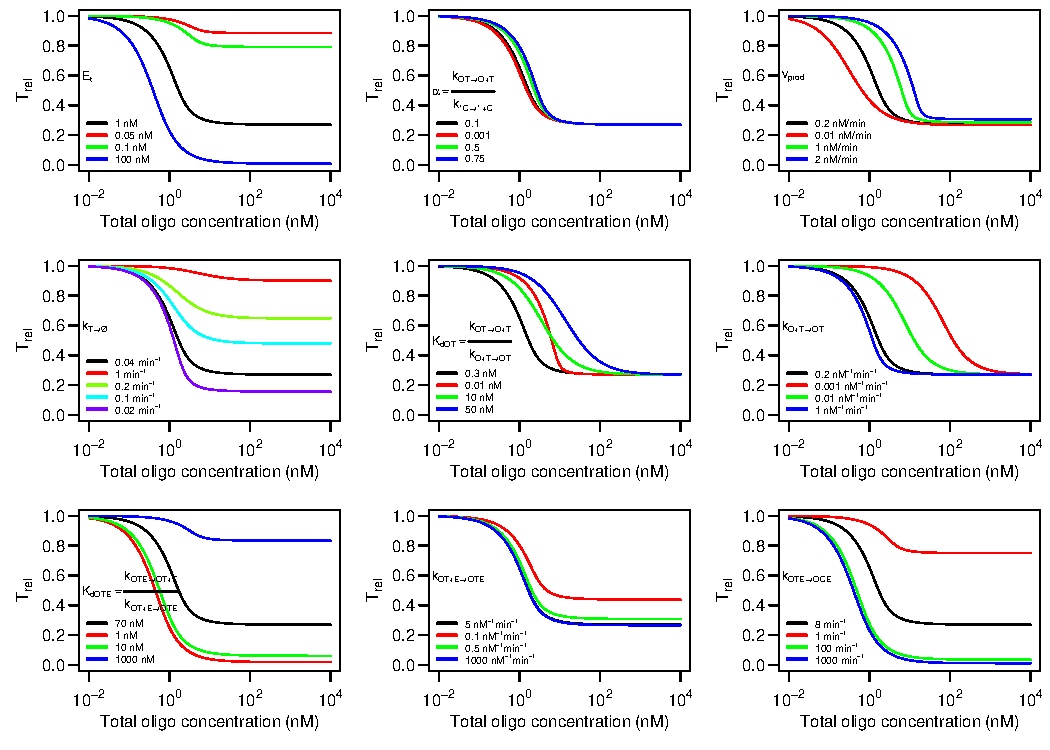
\includegraphics[width=\textwidth]{SuppFile1-S1.pdf}
\caption{Dose-response curves for different values of $E_{t}$, $\alpha$, $\vp$, $\vd$, $\KdOT$, $\kOpT$, $\KdOTE$, $\kt$, and $\kE$ (top,left to bottom,right). Black lines correspond to the parameter values listed in Supplementary Table.}\label{fig::Etot}
\end{figure}


%%%%%%%%%%%%%%%%%%%%%%%%%%%%%%%%%%%%%%%%%%%%%%%%%%%%%%%%%%%%%%%%%%%%%%%%%%%%%
\section{Supplementary Figure S2}
Using the R-function \texttt{drm()} from the drc package (v2.3-0) a dose-response curve is fitted to $\Trel$ as a function of $O_t$ to obtain an $\EC$-value. This is calculated through the R-function \texttt{EC50()} that takes $\KdOT$ and the set of parameters as input:
\begin{Schunk}
\begin{Sinput}
> EC50(KdOT=0.1,param=parms)
\end{Sinput}
\begin{Soutput}
    EC50 
1.218908 
\end{Soutput}
\end{Schunk}
For a range of $\KdOT$-values, the corresponding $\EC$-values can be calculated. These can be fitted to a parabola using the R-function \texttt{lm()}, see Supplementary Figure S2. 
\begin{Schunk}
\begin{Sinput}
> D1_seq <- 10^seq(-3,3.2,by=0.25)
> ECseq <- sapply(D1_seq,EC50)
> FitPar <- lm(log10(ECseq) ~ log10(D1_seq) + I(log10(D1_seq)^2))
\end{Sinput}
\end{Schunk}
\begin{figure}[!h]
\begin{Ncenter}
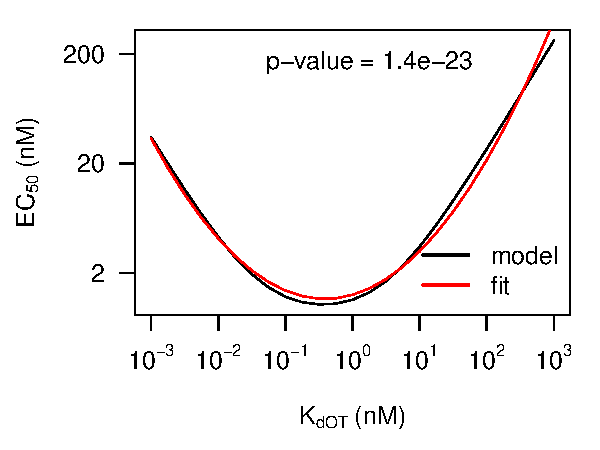
\includegraphics[width=0.6\textwidth]{SuppFile1-S31.pdf}
\end{Ncenter}
\caption{$\EC$ as a function of $\KdOT$ is fitted on a log-log scale to a parabola.}\label{fig::Optfit}
\end{figure}


%%%%%%%%%%%%%%%%%%%%%%%%%%%%%%%%%%%%%%%%%%%%%%%%%%%%%%%%%%%%%%%%%%%%%%%%%%%%%
\section{Supplementary Figure S3}
Supplementary Figure~\ref{fig::Opt} shows $\EC$ as a function of $\KdOT$ for various parameter values. It can be seen that the optimal affinity, quantified by $\KdOT$, changes as parameters are changed. A lower value of $\KdOT$ correponds to a better affinity for the oligonucleotide.
% % % %
% <<S2,echo=FALSE,fig=TRUE,include=FALSE,width=7,height=4>>=
% parc <- c('Et','alpha','vprod','KdOTE','kcleav','kdegrad')
% xlabl <- list(~nM,~phantom(0),~'nM/min',~nM,'/min','/min')
% xlabll <- list(~E[t],~alpha,~v[prod],~K[dOTE],~k[OTE%->%OCE],~k[T%->% Ø])
% parRange <- list(etot=c(0.01,1,10),alpha=c(0.005,0.01,0.95),
%                   vt=c(0.001,0.01,1.5),D2=c(0.5,10,100),
%                  kE=c(5,100,200),kd=c(0.005,0.05,0.5)) 
% D1_seq <- 10^seq(-3,3,by=0.25)
% EC50_fit <- as.list(1:length(parc))
% for(j in 1:length(parc)){
%  Lparseq <- parRange[[j]]
%  EC50_fit[[j]] <- matrix(NA, nrow=length(Lparseq),ncol=length(D1_seq))
%  
%  for(i in 1:length(Lparseq)){
%    parmsb <- parms; parmsb[parc[j]] <- Lparseq[i]
%    EC50_fit[[j]][i,] <- sapply(D1_seq,EC50,param=parmsb)
%  }
% }
% cbar <- c('orange','darkgreen','black')
% pdf('SuppFile1-S2.pdf',width=6.5,height=6.5)
% layout(matrix(c(1:6),3,2,byrow=T))
% for(j in 1:6){
%  Lparseq <- parRange[[j]]
% 
%  par(cex=0.75,mar=c(4,4,0.5,0.5),bty='o',mgp=c(2.2,0.7,0))
%  
%  for(i in 1:length(Lparseq)){
%    if(i==1){
%      plot(D1_seq,EC50_fit[[j]][1,],log='xy',panel.first=grid(col='grey',lty=3),
%            ylab=expression(EC[50]~' (nM)'),col=cbar[i],
%            ylim=c(1E-1,200),type='l',xaxt='n',yaxt='n',lwd=2,xlab=expression(K[dOT]~'(nM)'))
%      axis(1,at=c(1E-2,1,1E2),labels=pretty10expLP(10^c(-2,0,2),drop.1=T))
%      axis(2,at=c(1E-1,1,10,1E2),labels=pretty10expLP(10^c(-1:2),drop.1=T))
%    }else{
%      lines(D1_seq,EC50_fit[[j]][i,],col=cbar[i],lwd=2)
%     }
%   }
%   legend('bottomright',fill=cbar,cex=0.65,bg='white',x.intersp=0.2,
%           legend=as.expression(sapply(Lparseq,
%                            function(x) substitute(x*y,list(x=x,y=xlabl[[j]])))),
%           border=cbar,bty='o',box.lwd=0.5)
%   legend('top',as.expression(xlabll[[j]]),bty='n')
% }
% dev.off()
% % % @
% % 

\begin{figure}[!h]
\begin{Ncenter}
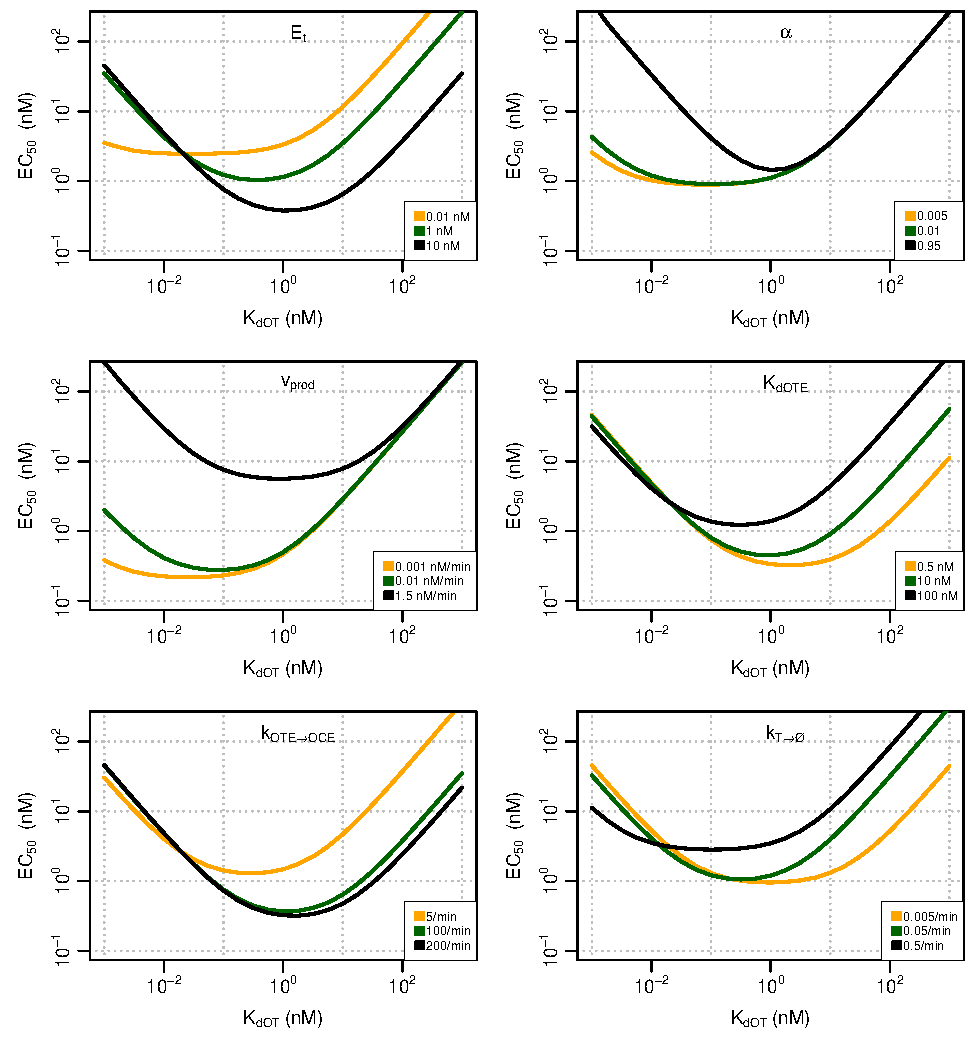
\includegraphics[width=\textwidth]{SuppFile1-S2.pdf}
\end{Ncenter}
\caption{The optimal affinity is dependent on the parameter settings. In the panels the $\EC$ concentration is plotted against the binding affinity, quantified by $\KdOT$, for various parameters. We have varied the total RNAse H concentration ($E_t$), $\alpha$, the target production ($\vp$), the dissociation constant for the OTE complex ($\KdOTE$), the rate of target cleavage ($\kE$),  and the target degradation ($\vd$).}\label{fig::Opt}
\end{figure}


%%%%%%%%%%%%%%%%%%%%%%%%%%%%%%%%%%%%%%%%%%%%%%%%%%%%%%%%%%%%%%%%%%%%%%%%%%%%%
\section{Supplementary Figure S4}
The stochastic simulation of the model is carried out by use of the \texttt{ssa()} R-function from the GillespieSSA package (v.0.5-4). The inputs to ssa are an initial state vector (x0), which is the initial number of molecules, a propensity vector (a), which denotes the different states of the system, a state-change matrix (nu), which is the change in number of molecule (rows) if a reaction occur (column), the model-parameters (parms) and the final time (tf).
\begin{Schunk}
\begin{Sinput}
> library(GillespieSSA)
> #Model parameters
> parms1 <- c(kOpT = 2E-5,kOTpE =50E-5 ,vprod = 150,  kdegrad = 0.04,		  
+               kcleav = 2, kOT =0.06, kOTE=2, kC = 0.1)
> #Initital state vector
> x0 <- c(Tt=parms1["vprod"]/parms1["kdegrad"],
+         OT=0,OTE=0,E=1e3,O=1e5,OCE=0,OC=0)
> names(x0) <- c('Tt','OT','OTE','E','O','OCE','OC')
> #Propensity vector
> a <-  c("vprod","kOpT*O*Tt","kdegrad*Tt","kOT*OT","kOTE*OTE","kdegrad*OT",
+         "kOTpE*OT*E","kdegrad*OTE","kcleav*OTE","kC*OC","kOTE*OCE" )
> #State-change matrix
> nu <- matrix(0,7,length(a))
> dimnames(nu) <- list(names(x0),a)
> #T
> nu['Tt',c('vprod','kOT*OT')] <- 1
> nu['Tt',c('kOpT*O*Tt','kdegrad*Tt')] <- -1 
> #OT
> nu['OT',c('kOpT*O*Tt','kOTE*OTE')] <- 1
> nu['OT',c('kOT*OT','kOTpE*OT*E','kdegrad*OT')] <- -1
> #OTE
> nu['OTE',c('kOTpE*OT*E')] <- 1
> nu['OTE',c('kOTE*OTE','kdegrad*OTE','kcleav*OTE')] <- -1
> #E
> nu['E',c('kOTE*OTE','kdegrad*OTE','kOTE*OCE')] <- 1
> nu['E',c('kOTpE*OT*E')] <- -1
> #O
> nu['O',c('kOT*OT','kdegrad*OTE','kdegrad*OT','kC*OC')] <- 1
> nu['O',c('kOpT*O*Tt')] <- -1
> #OCE
> nu['OCE',c('kcleav*OTE')] <- 1
> nu['OCE',c('kOTE*OCE')] <- -1
> #OC
> nu['OC',c('kOTE*OCE')] <- 1
> nu['OC',c('kC*OC')] <- -1
> #The Gillespie simulation
> Gillespie <- ssa( x0=x0,a=a,nu=nu,
+       parms = parms1,tf=1E3,method = "ETL")
\end{Sinput}
\end{Schunk}
% Check that $[O]+[OT]+[OTE]+[OCE]+[OC] = O_t$ at all times:
% <<echo=T>>=
% range(rowSums(Gillespie$data[,c('O','OT','OTE','OCE','OC')])-
%         x0['O'])
% @
% Check that $[E]+[OTE]+[OCE] = E_t$ at all times:
% <<echo=T>>=
% range(rowSums(Gillespie$data[,c('OTE','OCE','E')])-x0['E'])
% @
Supplementary Figure~\ref{fig:Trelstoc} shows $\Trel$ from the Gillespie simulation.
\begin{figure}[!h]
\begin{Ncenter}
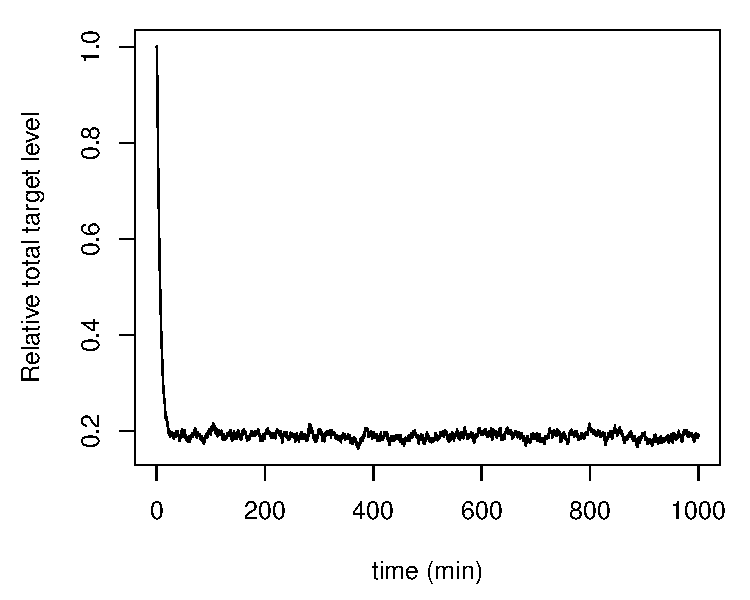
\includegraphics[width=0.6\textwidth]{SuppFile1-Trel.pdf}
\end{Ncenter}
\caption{The time-trace for the relative total target level when the model is simulated stochastically.}\label{fig:Trelstoc}
\end{figure}


%%%%%%%%%%%%%%%%%%%%%%%%%%%%%%%%%%%%%%%%%%%%%%%%%%%%%%%%%%%%%%%%%%%%%%%%%%%%%
\section{Supplementary Figure S5}
After a while the stochastic simulation reaches a plateau. In Supplementary Figure~\ref{fig:Trelstoc} the plateu starts around $50$min. The mean of $\Trel$ within the plateu is calculated through the R-function \texttt{Trelstoc()}. Using this function we can generate dose-response curves (Supplementary Figure~\ref{fig:stocEC50},left). From these $\EC$-values can be calculated using \texttt{EC50stoc()} and they are subsequently plotted as a function of $\kmo$ (Supplementary Figure~\ref{fig:stocEC50},right):
\begin{Schunk}
\begin{Sinput}
> #### Sequence of k(OT -> O+T) values
> lseq <- c(1,2.5,5,7.5)
> lKOT <- c(1E-3*lseq[-1],1E-2*lseq,1E-1*lseq)
> #### Generation of dose-response curves
> DRcurve <- lapply(lKOT,function(ki){ 
+             sapply(10^seq(2.5,6,by=0.2),
+                    function(i) Trelstoc(i,kOT=ki)$Tstat)})
> DRc <- lapply(DRcurve,function(x) x[,!is.na(x[3,])] )
> #### Calculation of EC50
> EC50_lKOT <- sapply(1:length(DRc),
+               function(x){EC50stoc(DRc[[x]][2,],DRc[[x]][1,])})
\end{Sinput}
\end{Schunk}
\begin{figure}[!h]
\begin{Ncenter}
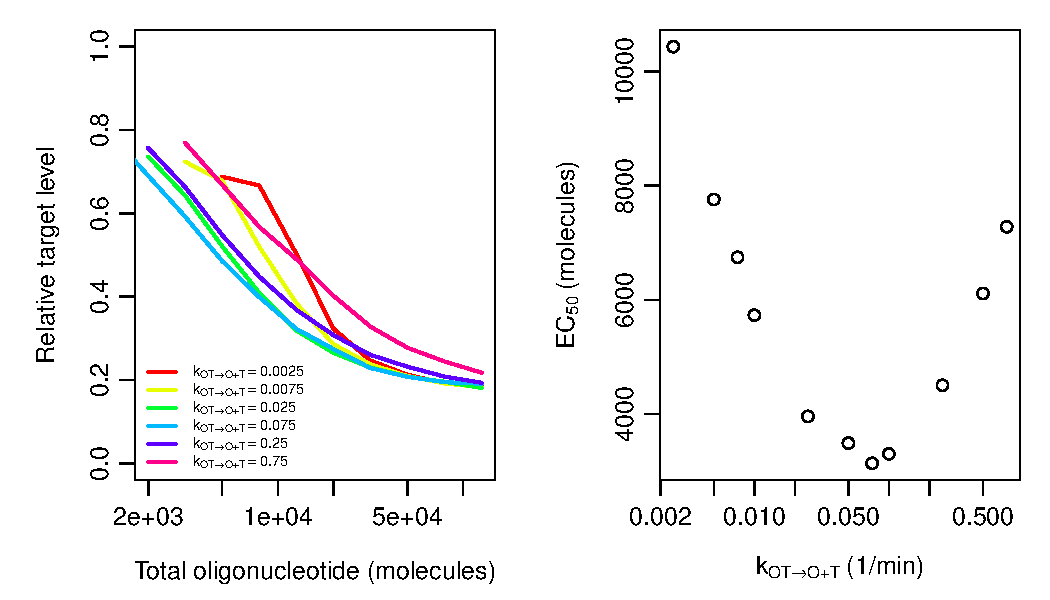
\includegraphics[width=\textwidth]{SuppFile1-EC50.pdf}
\end{Ncenter}
\caption{Left: Dose-response curves for various values of $\kmo$ (compare to Supplementary Figure S1,middle). Right: $\EC$ as a function of $\kmo$. A high value of $\kmo$ corresponds to a low affinity.}\label{fig:stocEC50}
\end{figure}
\newpage


%%%%%%%%%%%%%%%%%%%%%%%%%%%%%%%%%%%%%%%%%%%%%%%%%%%%%%%%%%%%%%%%%%%%%%%%%%%%%
\section{Supplementary Figure S6}
\begin{figure}[!h]
\begin{Ncenter}
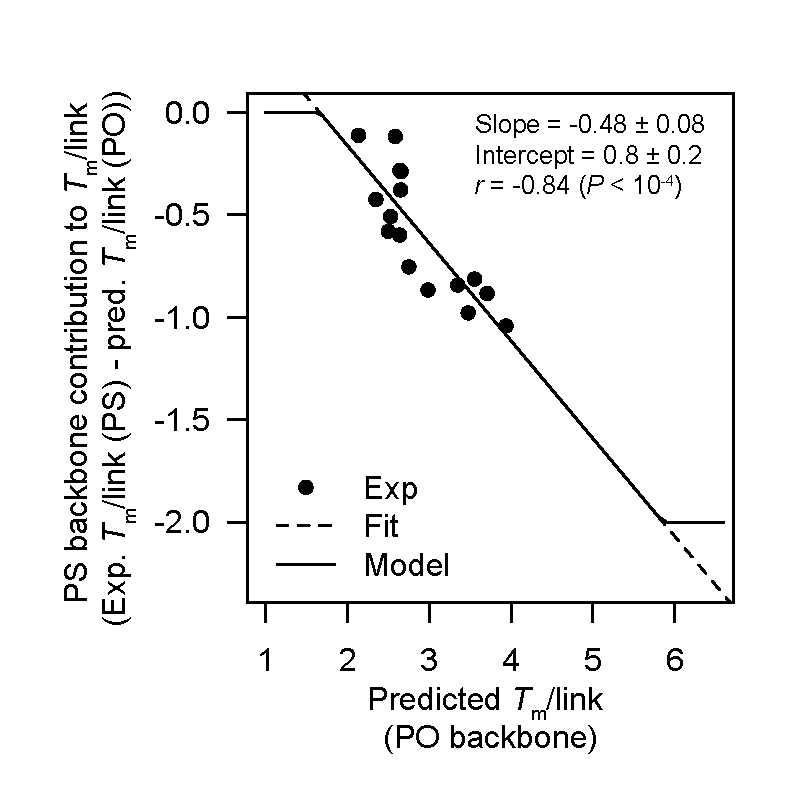
\includegraphics[width=0.65\textwidth]{SuppFig_PS.pdf}
\end{Ncenter}
\caption{The effect on $T_m$ of a phosphorothioate backbone was estimated using published data from Ref. \cite{Hashem:1998kf}.}\label{fig:figPS}
\end{figure}


%%%%%%%%%%%%%%%%%%%%%%%%%%%%%%%%%%%%%%%%%%%%%%%%%%%%%%%%%%%%%%%%%%%%%%%%%%%%%
\section{Supplementary Figure S7}
\begin{figure}[!h]
\begin{Ncenter}
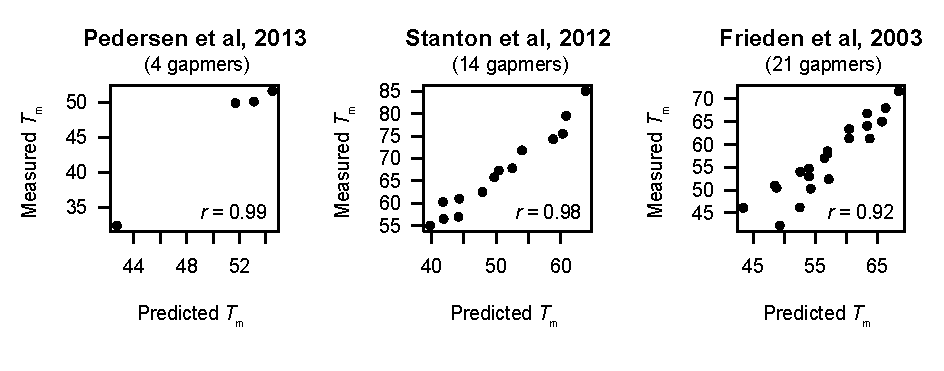
\includegraphics[width=\textwidth]{SuppFigS3.pdf}
\end{Ncenter}
\caption{Measured melting temperature versus predicted melting temperature. There are clear correlations ($r > 0.92$, $P < 0.01$, Pearson's correlation) between predicted and measured $T_m$. Pedersen et al: 4 LNA-modified oligonucleotides targeting apolipoprotein B (this work), Stanton et al: 14 LNA-modified oligonucleotides targeting the glucocorticoid receptor \cite{Stanton:2012fu}. Frieden et al: 21 LNA-modified oligonucleotides targeting the luciferase firefly gene \cite{Frieden:2003er}. Melting curves were recorded with a Perkin Elmer spectrophotometer. Oligonucleotide and its complementary RNA, both at 1.5$\mu M$, were dissolved in buffer (20mM phosphate buffer, 100mM NaCl, 0.1nM EDTA, pH 7). Samples were denatured at $95^\circ$C for 3min and slowly cooled to $20^\circ$C prior to measurements. Melting curves were recorded at 260nm using a heating rate of 1$^\circ$C/min, a slit of 2nm and a response of 0.2s. From this, $T_m$-values were obtained from the maxima of the first derivatives of the melting curves.}\label{fig:figTm}
\end{figure}

\newpage
\bibliography{ASOmodels}


\end{document}
